\documentclass{article}
\usepackage{graphicx,color}


\setlength{\textwidth}{6.5in}
\setlength{\textheight}{8.0in}
\setlength{\oddsidemargin}{0in}
\setlength{\evensidemargin}{0in}
\setlength{\parskip}{2ex}
\setlength{\parindent}{0in}

%To display answers, replace "white" with "red" here;
\newcommand{\answer}[1]{\color{red}#1}

\begin{document}
\pagestyle{myheadings}\markright{
CU Boulder \hspace{0.5in} MATH 2510 - Introduction to Statistics }

\begin{center}
\textbf{\underbar{In-class Worksheet 9}}
\end{center}

\begin{enumerate}

\item Given a normal curve (shown here),  what percentage of the area lies 

\begin{center}
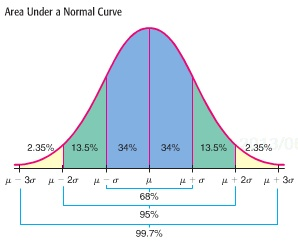
\includegraphics[scale=0.6]{WS10_NormalArea.jpg}
\end{center}

	\begin{enumerate}
	\item to the right of $\mu$? 
	
	{\answer The mean $\mu$ sits in the center of the data, so 50\% lies to the right (and to the left) of $\mu$.}
	
	\item between $\mu - \sigma$ and $\mu$? 
	
	{\answer The first region to the left of $\mu$ to $\mu-\sigma$ there is 34\% of the area.}
	
	\item between $\mu + \sigma$ and $\mu + 2\sigma$? 
	
	{\answer Looking at the graph, the region between $\mu + \sigma$ and $\mu +2\sigma$ consists of 13.5\% of the area.}
	
	\item between $\mu-2\sigma$ and $\mu + \sigma$? 
	
	{\answer For $\mu-2\sigma$ to $\mu + \sigma$ we can add the three percentages 13.5\%, 34\%, and 34\% to get 81.5\%.}
	
	\end{enumerate}
	
\item The incubation time for Rhode Island Red chicks is normally distributed with a mean of $\mu = 21$ days and a standard deviation of about $\sigma =1$ day.  If 1000 eggs are being incubated, how many chicks do we expect to hatch
	\begin{enumerate}
	\item on day 21 or after?
	
	{\answer Since $\mu = 21$, the percentage of the eggs that will hatch at that time or greater is 50\%.  So, that is 500 of the eggs.}
	
	\item between 20 and 21 days? 
	
	{\answer Since $\mu = 21$ and $\sigma =1$, we are looking at the percentage of the eggs in the interval $\mu-\sigma$ to $\mu$ which is 34\%.  So, that is 340 of the eggs.}
	
	\item between 22 and 23 days?
	
	{\answer Since $\mu = 21$ and $\sigma=1$, we are looking at the percentage of eggs in the interval $\mu+\sigma$ and $\mu + 2\sigma$ which is 13.5\%.  So, that is 135 of the eggs.}
	
	\item between 19 and 22 days?
	
	{\answer Since $\mu = 21$ and $\sigma=1$, we are looking at the percentage of eggs in the interval $\mu-2\sigma$ and $\mu + \sigma$ which is 81.5\%.  So, that is 815 of the eggs.}
	
	\end{enumerate}

\newpage

\item The Empirical Rule tells us the percentage of data values that lie within certain intervals about the mean when we have a normal distribution as follows.

\begin{center}
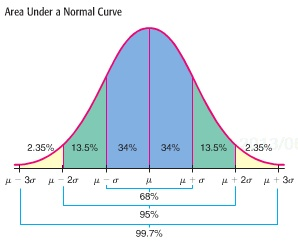
\includegraphics[scale=0.5]{WS10_NormalArea.jpg}
\end{center}

	\begin{enumerate}
	\item According to Chebyshev's Theorem, what is the minimum percentage of data that must lie within the interval $\mu-2\sigma$ to $\mu + 2\sigma$?  How does this compare to the results for the Empirical Rule?
	
	{\answer The result of Chebysev's Theorem is that at least $1-\frac{1}{2^2} = 75\%$ of the data fall within in the interval...and this is true for {\em any} data distribution.  \\
	For a normal distribution, the Empirical Rule shows us that there is approximate 95\% of the data falling within that same range.}
	
	\item The diagram for the Empirical Rule only accounts for 99.7\% of the data values.  Where do the remaining 0.3\% of the data fall?
	
	{\answer The remaining 0.3\% must lie outside the interval from $\mu-3\sigma$ to $\mu + 3\sigma$...That is, those data values lie fall out in the tails of the distribution.  Additionally, since the distribution is symmetric, half of them (or 0.15\%) lie below $\mu-3\sigma$ and the other half lie above $\mu + 3\sigma$.} 
	
	\item Keeping in mind that remaining 0.3\% of the data, what percentage of the data values lie to the left of $\mu-\sigma$?
	
	{\answer Add 13.5\%, 2.35\%, and 0.15\% to get 16\%. 
	
	Note that equivalently, since we know that 50\% lie to the left of the mean $\mu$ and 34\% lie between $\mu-\sigma$ and $\mu$, that leaves 16\% lying to the left of $\mu-\sigma$. }
	
	\item Keeping in mind that remaining 0.3\% of the data, what percentage of the data values lie to the left of $\mu+2\sigma$? 
	
	{\answer Add 13.5\%, 34\%, 34\%, 13.5\%, 2.35\%, and 0.15\% to get 97.5\%.
	
	Note that equivalently, since we know that 50\% lie to the left of the mean $\mu$ and $34\%+13.5\%$ lie between $\mu$ and $\mu+2\sigma$, that total is 97.5\% lying to the left of $\mu+2\sigma$. } 
	\end{enumerate}

\item In preparation for Sections 6.2 and 6.3, suppose the mean of a normal distribution is $\mu = 75$ with a standard deviation of $\sigma = 8$.  For each of the following values of the random variable $x$, determine whether $x$ is above or below the mean and then determine the number of standard deviations away from the mean that $x$ lies.  (Note that your second answer could be a fraction or decimal number.)

	\begin{enumerate}
	\item $x=83$ 
	
	{\answer $x=83$ is above the mean of $\mu = 75$.  Specifically, $\frac{83-75}{8} = 1$.  So, $x$ is 1 standard deviation above the mean.}
	\item $x=51$ 
	
	{\answer $x=51$ is below the mean of $\mu = 75$.  Specifically, $\frac{51-75}{8} = -3$ .  So, $x$ is 3 standard deviations below the mean.}
	\item $x=79$ 
	
	{\answer $x=79$ is above the mean of $\mu = 75$.  Specifically, $\frac{79-75}{8} = 0.5$.  So, $x$ is $0.5$ standard deviations above the mean.}
	\item $x=65$ 
	
	{\answer $x=65$ is below the mean of $\mu = 75$.  Specifically, $\frac{65-75}{8} = -1.25$.  So, $x$ is $1.25$ standard deviations below the mean.}
	\end{enumerate}

\vfill

\item Hydraulic pressure in the main cylinder of the landing gear of a commercial jet is very important for a safe landing.  In-flight landing tests show that the actual pressure in the main cylinders is variable (approximately normal) with a mean of 819 pounds per square inch and a standard deviation of 23 pounds per square inch, which are considered safe.

Two different planes were tested with 10 test-landings.  Here are the recorded pressures for each. 

Plane A 

\begin{tabular}{l|cccccccccc}
\hline 
Landing number  & 1& 2 & 3 & 4 & 5 & 6 & 7 & 8 & 9 & 10 \\
\hline
Pressure & 870 & 855 & 830 & 815 & 847 & 836 & 825 & 810 & 792 & 820 \\
\hline
\end{tabular}

Plane B 

\begin{tabular}{l|cccccccccc}
\hline 
Landing number  & 1& 2 & 3 & 4 & 5 & 6 & 7 & 8 & 9 & 10 \\
\hline
Pressure & 865 & 850 & 841 & 820 & 815 & 789 & 801 & 765 & 730 & 725 \\
\hline
\end{tabular}

	\begin{enumerate}
	\item  Is the pressure for Plane A ``in control" or not?  If not, describe the specific out-of-control signals present. 
	
	{\answer Out of control Signal 1: $\mu -3\sigma = 750$ and $\mu +3\sigma = 888$.  No values fall outside that range. 
	
	Out of control Signal 2 : $\mu = 819$.  There are no more than 3 consecutive values above $\mu$ and no more than 2 consecutive values below $\mu$.
	
	Out of control Signal 3: $\mu -2\sigma = 773$ and $\mu +2\sigma = 865$.  There is only 1 value that lies beyond either end of that range, so certainly not 2 of 3 consecutive values do. There are no out-of-control warning signals present for Plane A.} 
	
	\item  Is the pressure for Plane B ``in control" or not?  If not, describe the specific out-of-control signals present.
	
	{\answer Out of control Signal 1: $\mu -3\sigma = 750$ and $\mu +3\sigma = 888$.  There are two values that fall below 750. 
	
	Out of control Signal 2 : $\mu = 819$.  There are no more than 4 consecutive values above $\mu$ and no more than 6 consecutive values below $\mu$. 
	
	Out of control Signal 3: $\mu -2\sigma = 773$ and $\mu +2\sigma = 865$.  The last three values recorded lie below 773, so there are two occasions of 2 out of 3 consecutive values flying beyond the $2\sigma$ level on the same side. There are two out-of-control warning signals present for Plane B.} 
	\end{enumerate}
	
	
\end{enumerate}

\vfill

\end{document}

